%\todofilebegin{030\_sos\_model.tex}
%%%%%%%%%%%%%%%%%%%%%%%%%%%%%%%%%%%%%%%%%%%%%%%%%%%%%%%%%%%%%%%%%%%%%%%%%%%%%%
%%%%%%%%%%%%%%%%%%%%%%%%%%%%%%%%%%%%%%%%%%%%%%%%%%%%%%%%%%%%%%%%%%%%%%%%%%%%%%
%%%%%%%%%%%%%%%%%%%%%%%%%%%%%%%%%%%%%%%%%%%%%%%%%%%%%%%%%%%%%%%%%%%%%%%%%%%%%%

\section{The Design and Architecture of SOS}


\subsection{The Need to Observe Locally}

%%%%%
Because the features we are interested in are going to emerge at run
time, it is necessary to obtain observations of real-world
applications, libraries, data transmissions, and hardware state.
%
To realize a model for performance that is practically suited for
exascale architecures, it is further necessary to collect and analyze
information as close as possible to its source, and to accept metrics
submitted from an arbitrary array of sources.
%
This in situ runtime design effectively parallelizes the execution of
the observation system and gives opportunities to cut down on
coordination overhead when providing mechanisms for on-line feedback
and control.
%%%%%


%-----------------------------------------------------------------------------

\subsection{What is Observed}

%%%%%
\textit{``We'll have to know EVERYTHING if we're going to bother trying to
know anything at all.''}
%%%%%

%%%%%
At a low-level, HPC computer engineering has grown in complexity and
sophistication, and many on-core processor behaviors that used to be
isolated, synchronous, and predictable, are now interrelated,
data-dependant, asynchronous, and demonstrate variations in
performance impossible to comprehensively characterize a priori.
%
As core transistor density increases on the nodes of a cluster, and
the mean number of cores per node also increases, the unpredictability
and inconsistency of the hardware itself becomes an increasingly
significant contributor to observed variability.
%
Hardware is an important source to consider when it comes to
performance because almost nothing that can be done to control for it
or eliminate it, the noisey results derived from noisy hardware has to
be admitted in the results, and therefore keeping track of
\textit{when and where}, not merely how, a program ran is growing in
significance to all HPC experiments with an interest in improving
performance.
%%%%%

%%%%%
Performance of HPC codes can be impacted from many different sources:
\begin{itemize}
      %
    \item Versions of software libraries across can differ across
      clusters, or even the same cluster across time.
      %
    \item Tuning factors to extract maximum performance from a code
      can vary across clusters, even if the code and the data do not
      change.
      %
      Shared filesystem performance, data transport methods,
      available per-process memory, co-processor presence and
      architecture, ...and more, all can be responsible for
      influencing sensitivity to novel tuning factors.
      %
    \item Concurrent activity elsewhere on the same cluster, activity
      that will necessarily vary between every iteration of the
      workflow, may be having a significant impact on observed
      performance.
      %
    \item At extreme scales, parts of a simulation are almost
      guaranteed to fail due to the marginal failure rates of hardware
      components approaching absolute certainty as the number of
      involved components increases.
      %
      These failures cannot be accurately predicted a priori, and
      the design constraints that account for and respond to them
      introduce performance perturbation and further complexity.
      %
\end{itemize}
%%%%%

%-----------------------------------------------------------------------------

\subsection{How to Observe}
%%%%%
SOSflow has been designed as a voluntary-participation runtime system
that runs in user space on commodity HPC platforms.
%
A daemon process is launched on node that acts as an intelligent
unbounded asynchronous hub for in situ collection of data from
multiple sources, the migration of that data into searchable stores,
and the targeted delivery of feedback messages from online analytics
modules observing the flow of information.
%%%%%

\subsubsection{``Put the Data Somewhere Useful''}
%%%%%
Because of the variety of metrics of interest, the fact that they may
not always be expressed in any given runtime, and that all possible
metrics are not known a priori to be hardcoded into a system, it is
exceedingly helpful from an architectural point of view if performance
observations are gathered into a common fabric from all sources.
%
Any well-meaning self-optimizing programm spinning opaque snapshots of
its internal state out into a proprietary database is denying all
other parts of the environment the ability to learn more about each
other, themselves, and that program.
%%%%%


\subsubsection{Simple, Clean, Universal}
%%%%%
Rather than seeing yet another printf()-style instrumentation
dead-end, or a Titanic-scale solution that requires deep federal
pockets or administrator priveleges to use, a well-designed
observation system will provide a clean and flexible interface
suitable for capturing and annotating metrics within their context,
and will bring the metrics from all sources together to be operated
over following a shared set of action-oriented semantics.
%
As users operating with self-interest will be the pioneers seeding
these raw data fields, the system should be easy to use and
accessible, and provide immediate benefit to anyone who wishes to add
some sweat equity.
%%%%%



%%%%%%%%%%%%%%%%%%%%%%%%%%%%%%%%%%%%%%%%%%%%%%%%%%%%%%%%%%%%%%%%%%%%%%%%%%%%%%
%%%%%%%%%%%%%%%%%%%%%%%%%%%%%%%%%%%%%%%%%%%%%%%%%%%%%%%%%%%%%%%%%%%%%%%%%%%%%%
%%%%%%%%%%%%%%%%%%%%%%%%%%%%%%%%%%%%%%%%%%%%%%%%%%%%%%%%%%%%%%%%%%%%%%%%%%%%%%

\section{SOS: Scalable Observation System}

%%%%%
SOS is concieved of as an architectural addition to the general fabric
of exascale clusters.
%
It is intended to be a widely-integrated service that evolves
low-level optimizations over time, with a broad set of functionality
that is available to all users of an exascale cluster.
%
It should feel like a tool meant for any developer's hands, not only
the performance researcher's.
%
If SOS is not to be doomed to gather dust on the shelf in obscurity,
it really only needs to do one thing: It needs to help.
%%%%%

%-----------------------------------------------------------------------------

\subsection{SOSflow}
%%%%%
Applying the semantic performance model to actual run-time
environments necessitated the development of new infrastructure
software, and so the second contribution to the general challenges of
monitoring scientific workflows is the SOSflow middleware.
%
SOSflow is designed to:
%
\begin{enumerate}
      %
    \item Facilitate on-line capture of performance data and various system
      events in situ (i.e. ``on node'') from arbitrary sources and
      perspectives at the same time.
      %
    \item Annotate the gathered data's semantic meaning with
      expressive ``high-level'' tags that facilitate contextualization
      and introspective analytics.
      %
    \item Store the captured data on node in a way that can be
      searched with dynamic queries in real-time as well as being
      suitable for long-term centralized archival.
      %
\end{enumerate}
%%%%%

%%%%%
SOSflow is divided into several components.  The core components are:
%
\begin{itemize}
      %
    \item \textbf{libsos} - Library of common routines for interacting with
      sosd daemons and SOS data structures
      %
    \item \textbf{sosd(listener)} - Daemon process running on each node
      %
    \item \textbf{sosd(db)} - Daemon process running on dedicated resources
      that stores data aggregated from one or more in situ daemons
      %
    \item \textbf{sosa} - Analytics framework for online query of SOS data
      %
\end{itemize}
%%%%%

%%%%%
Some accessory components are:
%
\begin{itemize}
    \item \textbf{sosd\_probe} - Collect real-time statistics from the daemon about
      its internal state and operating workload
      %
    \item \textbf{sosd\_stop} - Signal the SOSflow runtime to store its queues and
      safely shut down
      %
    \item \textbf{proc\_app} - Collect node runtime information from
      the /proc API on the node, submitting it to the daemon in the
      form of a publication
      %
    \item \textbf{demo\_app} - Benchmarking tool for testing SOSflow
      %
    \item \textbf{SOApy} - Python scripts for querying the SOS databases and plotting
      graphs from the results
      %
    \item \textbf{synthetic\_flow} - Tool for generating SOSflow-instrumented
      synthetic workflow of components using ADIOS+FlexPath
      that self-assemble into an arbitrary  user-specified DAG of
      data-dependent processing relations
      %
\end{itemize}
%%%%%

%%%%%
\subsection{SOSflow: Behavior}
%
The sosd daemon is itself an MPI application, and it is launched as a
background process in user space at the start of a job script, before
the scientific workflow begins.
%
The daemon first goes through a coordination phase where they performs
an MPI\_Allreduce() with all other daemon ranks in order to share
their role (DAEMON, DB, or ANALYTICS) and the name of the host they
are running on.
%
During the coordination phase, listener daemons select the sosd(db)
aggregate database that they will target for automatic asynchronous
transfer of the data they capture.
%
At present, the ranks of sosd(listener) use a simple round-robin
selection method to pick their database target.
%
All the sosd instances split up the total numeric space from 0 to
UINT64\_MAX for use in assigning globally unique ids (GUIDs).
%
All entries in the SOSflow system from that point forward are, if
appropriate, assigned a GUID such that uniqueness and provenance is
preserved even if queries straddle multiple data stores, or all data
stores are eventually synthesized into a global store.
%%%%%

%%%%%
\begin{figure*}[!t]
  \centering
  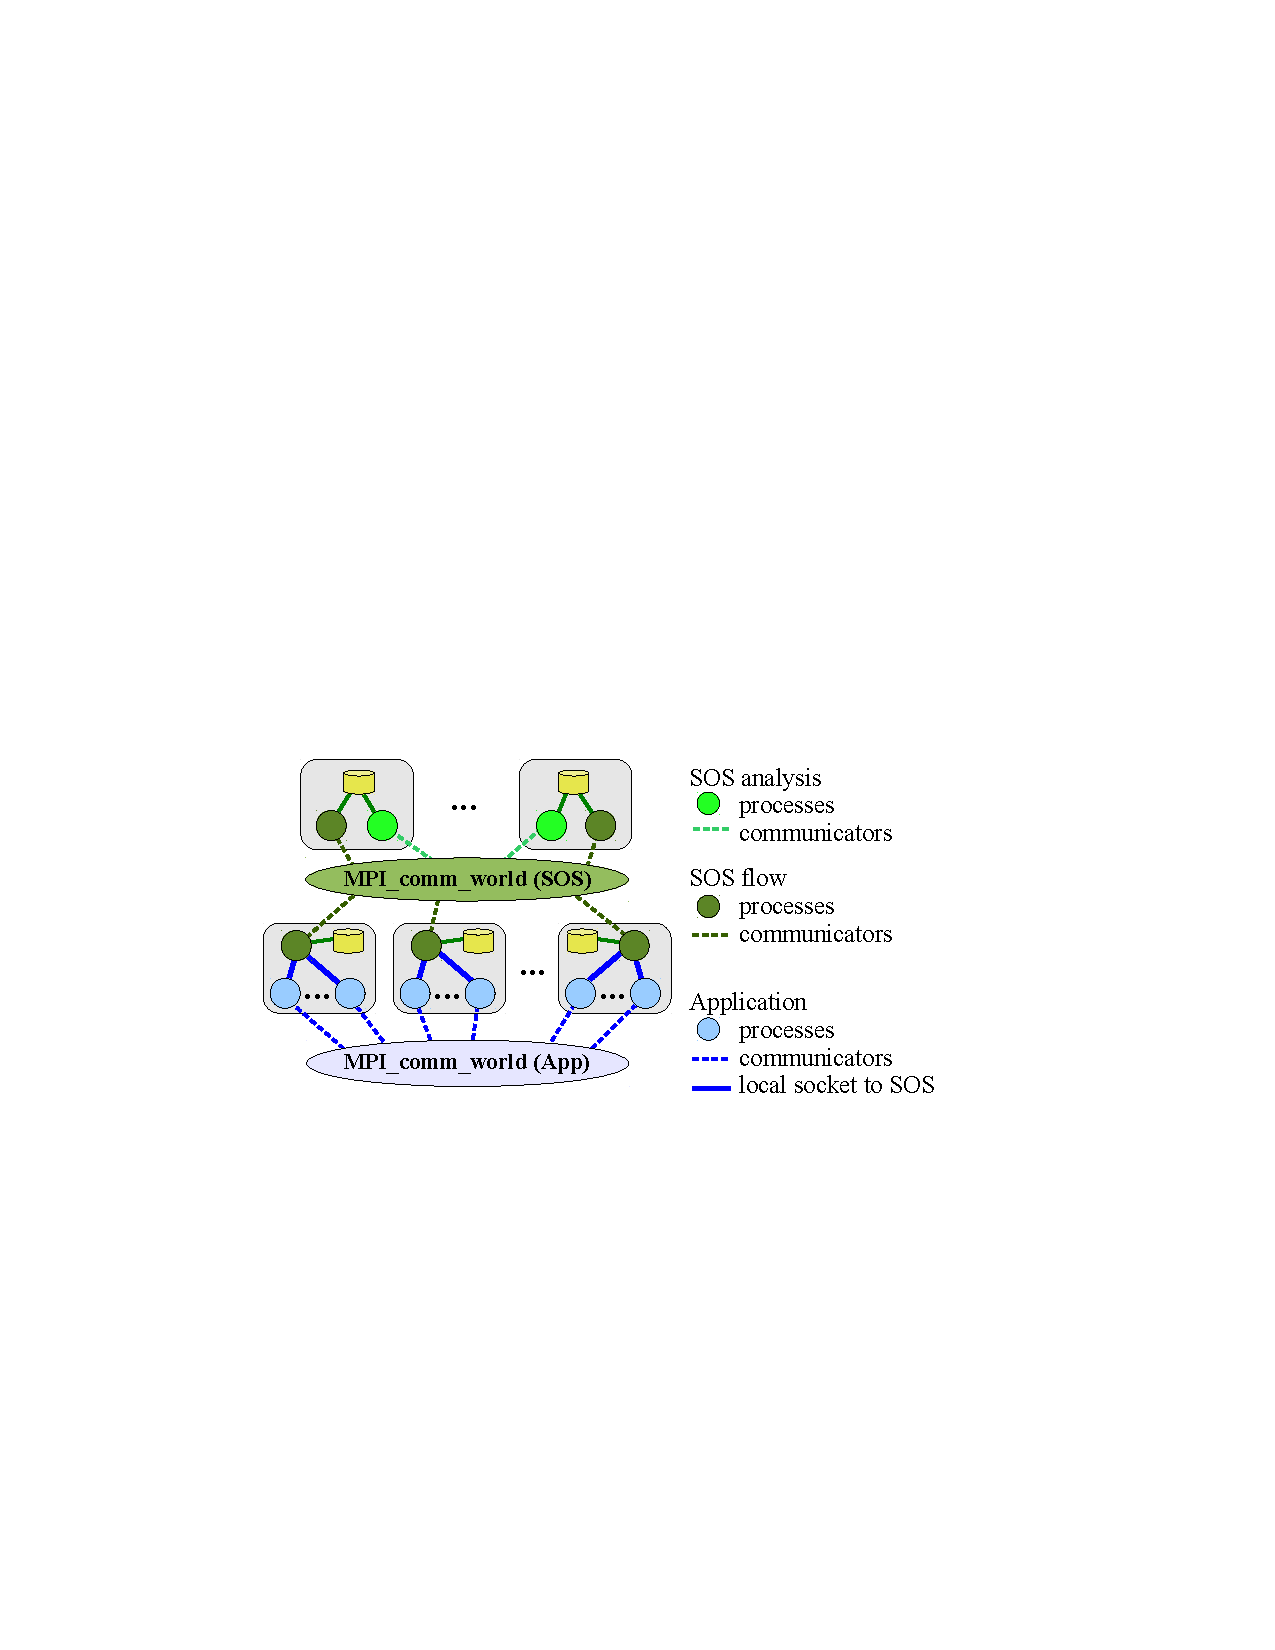
\includegraphics[width=5in]{images/sos-mpmd.pdf}
  \caption{SOSflow Communicates w/MPI and Sockets}
  \label{fig_sim}
\end{figure*}
%%%%%

%%%%%
Analytics modules use this time to determine if they are co-located
with a sosd(db) role, and set an internal flag that allows analytics
developers to branch their logic (if desired) between local instances that
can more quickly coordinate queries with the aggregate database, and any 
other optional independent ranks that are running on dedicated resources
for the purpose of doing calculations or rendering visualizations.
%
After having coordinate with the sosd ranks, sosa ranks split off into
their own private communicator, allowing the developer of a given sosa
module to utilize the collective communication benefits of the HPC
platform they are deployed on.
%%%%%

%%%%%
Once all of the sosd and sosa ranks are initialized and aware of each
other, they begin operating autonomously and no longer exchange global
collective messages -- all MPI messages are now point-to-point.
%
The sosd(listener) in situ daemons go into a loop listening to a
node-local TCP socket (specified by the SOS\_CMD\_PORT environment
variable) for messages from utilities or SOSflow-enabled source
applications.
%
sosd(db) database daemons do not monitor any socket at this time, but
rather are contacted exclusively through their MPI communicator.
%
When an analytics module submits a query, it does not address the
database files directly, but sends its query to the sosd(db) instance
over MPI\_COMM\_WORLD and receives results back as an MPI message
which is transparently parsed into an row and column iteratable
(SOS\_results *) table.
%%%%%

%%%%%
On node, the sosd(listener) program accepts single messages at a time
and immediately services them, as far as the message sender is aware,
quickly responding with a simple ACK message or with the data that was
requested.  This behavior follows a very simple stateless protocol
that exists between the daemon and its on-node clients.
%%%%%

%%%%%
\begin{figure*}[!t]
\centering
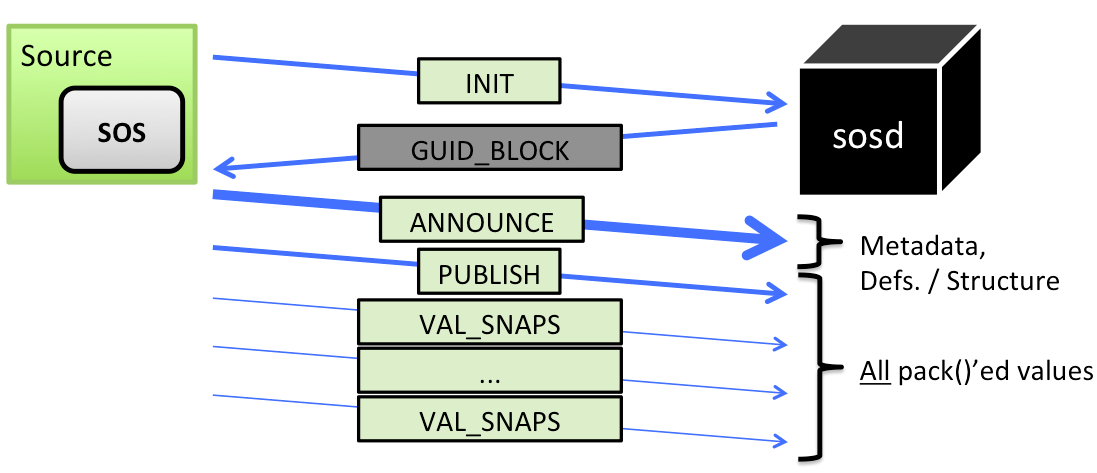
\includegraphics[width=5in]{images/sosd_protocol.png}
\caption{In Situ Client/Daemon Communication Protocol}
\label{fig_sim}
\end{figure*}
%%%%%

%%%%%
Messages are read off the socket rapidly and placed in the daemon's
unbounded asynchronous thread-safe queues to be processed by the
daemon's local\_sync and cloud\_sync threads.
%
The socket is nearly immediately clear for the next queue'd message to
be received.
%
Communication with the sosd(listener) is always initiated by the
clients.
%
Client applications do not need to monitor a socket, though certain
SOS client roles can spawn a lightweight background thread that
periodically checks in with their local daemon to see if any feedback
has been sent to that application, allowing for run-time adaptivity to
be decoupled from the application's schedule for transmitting its
information to SOSflow.
%%%%%

%%%%%
All of the communication functions in the sos client library are
handled transparently, SOS users need only interact with a simple API
to define and store values that they can then publish up to the daemon
as appropriate.
%
The protocols and the codes of the client library are designed to be
fast and minimize resource usage, though they will buffer values for
the user if they choose to hold them and only transmit to the daemon
at intervals.
%
It is very uncommon to see the blocking socket transmission calls
within SOS\_announce() and SOS\_publish() take longer than 0.002
seconds, in any of our testing scenarios. Calls to the more frequently
used SOS\_pack() value storage/update routine create no noticable
overhead at all when not used in the innermost loops of intense
computation, often returning in less than 0.0001 seconds even for very
large data sets.
%
When a client first registers with the sosd(listener) during
SOS\_init(), the daemon will assign that client library a break of
GUIDs to manage internally, so that many different client activities
can be handled correctly with no need for immediate interaction with
the daemon.
%
When a client library runs out of GUIDs it simply pings the daemon and
asks for more.
%%%%%

%%%%%
The typical order of API calls in a client is:
%
\begin{enumerate}
      %
    \item SOS\_init();
      %
    \item SOS\_pub\_create();
      %
    \item SOS\_pack();
      %
    \item SOS\_announce();
      %
    \item SOS\_publish();\\
    \dots\\
    \dots\\
      %
    \item SOS\_finalize();
      %
\end{enumerate}
%%%%%

%%%%%
\begin{figure*}[!t]
\centering
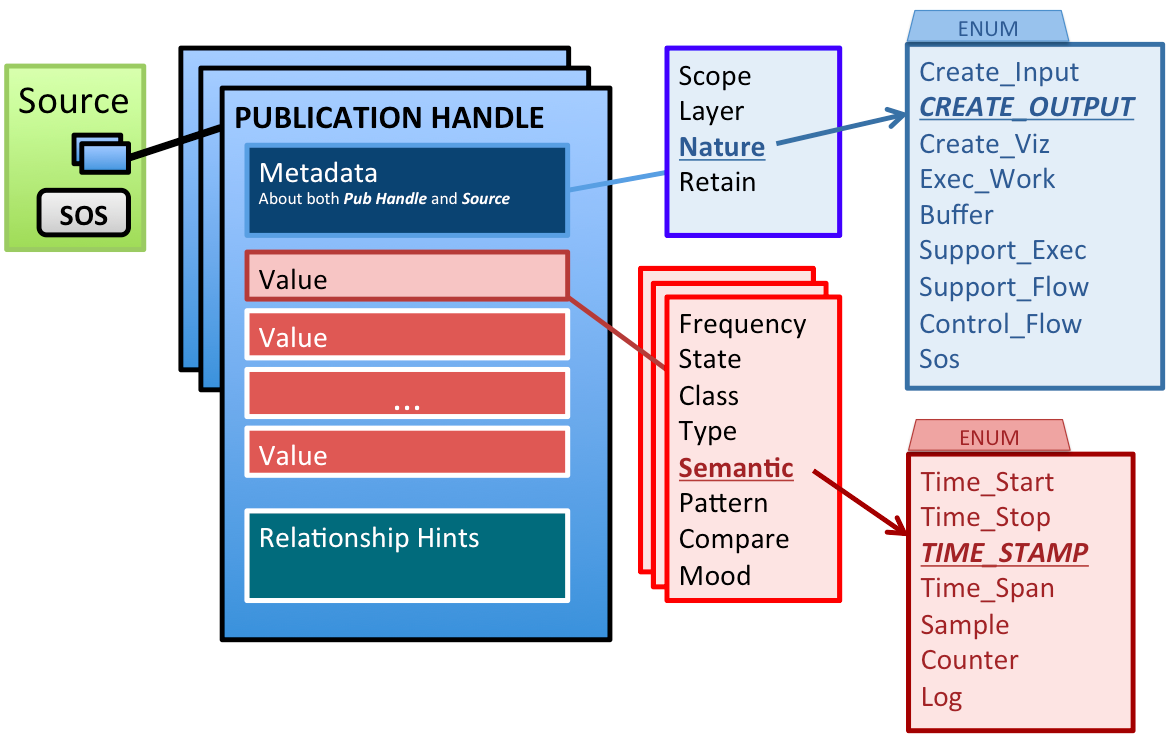
\includegraphics[width=5in]{images/pub_handle.png}
\caption{Structure of an SOS Publication Handle}
\label{fig_sim}
\end{figure*}
%%%%%

%%%%%
Data from clients in SOSflow is stored in a (SOS\_pub *) ``pub handle''
object.
%
This object organizes all of the application context information and
value-specific metadata, as well as managing the history of updates to
a value pending pending transmission to a sosd(listener), called
\textit{value snapshots}.
%
Every value that is passed through the SOSflow API is preserved and
eventually stored in a searchable database, along with any updated
metadata such as its timestamp tuples.
%
Multiple updates to the same value prior to a call to SOS\_publish()
are no exception, prior value snapshots are queued up and faithfully
transmitted along with the most recent update to that value.
%%%%%

%%%%%
\begin{figure*}[!t]
\centering
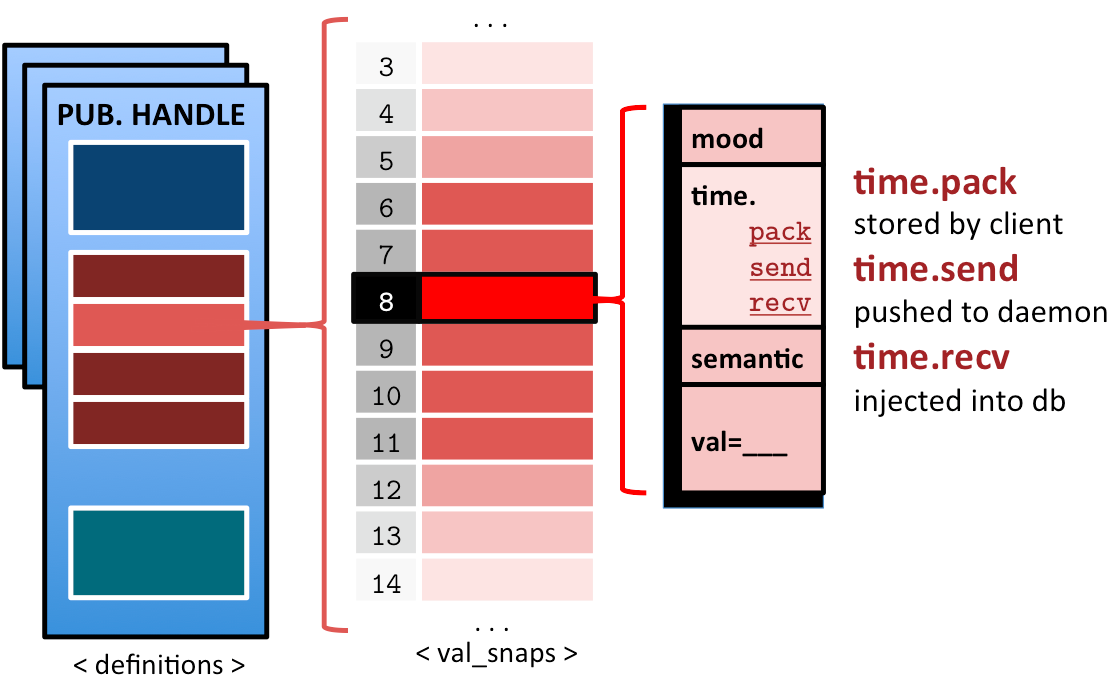
\includegraphics[width=5in]{images/val_snaps.png}
\caption{Complete History of For All Values, Including Metadata}
\label{fig_sim}
\end{figure*}
%%%%%

%%%%%
SOSflow is not a pure publish/subscribe system, the SOS\_announce()
function and its associated message type exist (for now) to seperate the
transmission of metadata apart from the transmission of the typically
more compact values stored in a pub.
%
Calling the SOS\_announce() function is entirely optional, though
never harmful, and good developer hygene in case it is not optional at
some point in the future.
%
If a pub handle has not been announced when it is passed to the
publish function, it with automatically recurse into the announce
function on your behalf.
%
Additionally, if you have added new value names, and not merely packed
updates to some previously announced values, the next time you
publish, those new value names will automatically be announced.
%%%%%

%%%%%
SOSflow is entirely thread-safe within the client application so long
as data elements are accessed only through the public API.
%
You could, if you for some reason wanted to, share a pub handle
between two threads: the system is designed to efficiently shield
users from the complexity of managing its state.
%
It is also designed to be as simple as possible without losing
flexibility.
%
When a value is packed into a pub handle, for the first time, that
effectively defines the value and configures it with a totally safe
set of metadata defaults.
%
If inspired to, a developer using SOSflow could then go render the
metadata more precise, though such noble pursuits are entirely
optional.
%
Data is thus defined to the system the same way it is updated in the
system, through the SOS\_pack() function.
%%%%%

%%%%%
The in situ sosd(listener) daemon does not keep track of applications,
and so does not know (or care) when they terminate.
%
The call to SOS\_finalize() provides a simple and clean way to clean
up SOS's internal memory objects and buffers, join any threads it may
have needed to spawn, and otherwise put things back how it found them
when SOS\_init() was called.
%
In the near future it is expected that SOS\_finalize() \textbf{will}
message the daemon, and so client applications should always make an
effort to call this function explicitly.
%%%%%

%%%%%
\subsection{SOSflow: Implementation}
%
\begin{itemize}
      %
    \item \textbf{Language}: C99
      %
    \item \textbf{External Requirements}:
      %
      \begin{itemize}
            %
          \item CMake
            %
          \item Pthreads
            %
          \item MPI
            %
          \item Sqlite3
            %
      \end{itemize}
      %
  \item \textbf{Key Source Files}: See Table 1.
    %
\end{itemize}
%%%%%

\begin{table}[!t]
%% increase table row spacing, adjust to taste
\renewcommand{\arraystretch}{1.3}
\caption{Key Source Files for SOSflow}
\label{tableexample}
\centering
\begin{tabular}{|c|c|}
\hline %%%%%%%%%%%%%%%%%%%%%%%%%%%%%%%%%%%%%%%%%%%%%%%%%%%%%%%%%
sos.h / sos.c & core functions of SOSflow\\
\hline %%%%%%%%%%%%%%%%%%%%%%%%%%%%%%%%%%%%%%%%%%%%%%%%%%%%%%%%%
sosd.h / sosd.c & SOSflow daemon\\
\hline %%%%%%%%%%%%%%%%%%%%%%%%%%%%%%%%%%%%%%%%%%%%%%%%%%%%%%%%%
sosa.h / sosa.c & SOS analytics core utilities\\
\hline %%%%%%%%%%%%%%%%%%%%%%%%%%%%%%%%%%%%%%%%%%%%%%%%%%%%%%%%%
sos\_debug.h & Debugging off / on (level) knobs\\
\hline %%%%%%%%%%%%%%%%%%%%%%%%%%%%%%%%%%%%%%%%%%%%%%%%%%%%%%%%%
demo\_app.c & Synthetic app for profiling SOSflow\\
\hline %%%%%%%%%%%%%%%%%%%%%%%%%%%%%%%%%%%%%%%%%%%%%%%%%%%%%%%%%
sosd\_cloud\_mpi.c & Off-node transport, coordination\\
\hline %%%%%%%%%%%%%%%%%%%%%%%%%%%%%%%%%%%%%%%%%%%%%%%%%%%%%%%%%
sosd\_db\_sqlite.c & Database operations\\
\hline %%%%%%%%%%%%%%%%%%%%%%%%%%%%%%%%%%%%%%%%%%%%%%%%%%%%%%%%%
\end{tabular}
\end{table}


%-----------------------------------------------------------------------------
\subsection{SOSa : Analytics}

%%%%%
SOSflow supports online query and analysis of the information that is
published into it.
%
Users of SOS are able to quickly write their own analytics modules
building by expanding from the provided templates.
%
When the sosd daemons are brought online, analytics modules are also
activated using MPMD syntax to add them to the daemon's mpirun
invocation.
%
Multiple analytics modules can be launched at once, so long as they
define unique SOSA\_MODULE\_COLOR values.
%
These unique 'colors' are used to split each analytics group into its
own communicator so the analytics codes can benefit from the HPC
resources of the job allocation to perform their work without engaging
with any other parts of SOSflow.
%
Queries are written in the dialect of SQL supported by the daemon, and
in the current case this is the fairly standard version in Sqlite3.
%
The query submitted as a string in a character array, and a special
(SOS\_results *) object is returned:
%%%%%

%%%%%
\begin{lstlisting}[frame=single, basicstyle=\small]
typedef struct {
    SOS_runtime *sos_context;
    int          col_max;
    int          col_count;
    char       **col_names;
    int          row_max;
    int          row_count;
    char      ***data;
} SOSA_results;

SOSA_results *results;                                                                                                                       
SOSA_results_init(SOS, &results);
char *query =
    "SELECT "
       "max(rowid), "
       "time_pack, "
       "time_recv "
    "FROM tblvals;";

SOSA_exec_query(query, results);

SOSA_results_output_to(fptr,
    results,
    "latency",
    SOSA_OUTPUT_W_HEADER);
\end{lstlisting}
%%%%%

%%%%%
There are utility functions to reset and destroy SOS\_results objects,
output them as CSV tables of JSON object lists, etc.
%
The full API for developers of analytics modules is available in the
sosa.h header file.
%%%%%

%%%%%
Queries are submitted to an aggregator daemon that your analytics
module is targeting.
%
sosd(db) ranks and sosa modules can be pinned to the same physical
node together at invocation, and analytics modules will favor the
sosd(db) rank they share a node with in order to enable fast in-memory
messaging rather than sending query results across the shared network
resources.
%
Queries are entirely arbitrary, and are allowed to examine the full
scope of data that has been submitted to the SOSflow runtime, from
whatever source derived.
%
At this time there are no security measures to prevent analytics
modules from accessing specific regions of the data, since all of the
data available in the database will have come from a user's own
applications.
%
This is a section of the SOSflow development that is relatively novel,
and has not been implemented with much optimization in place.
%
When a query is executed it locks the database to prevent other
threads from writing to it.
%
It is possible to write very inefficient queries that tie up the
database and create latency in the asynchronous queues.
%
Avoiding such issues is an exercise left to developers at this time,
though re-architecting this component of SOSflow is a high priority
for the next phases of its maturation.
%%%%%

%%%%%
\begin{figure*}[!t]
  \centering
  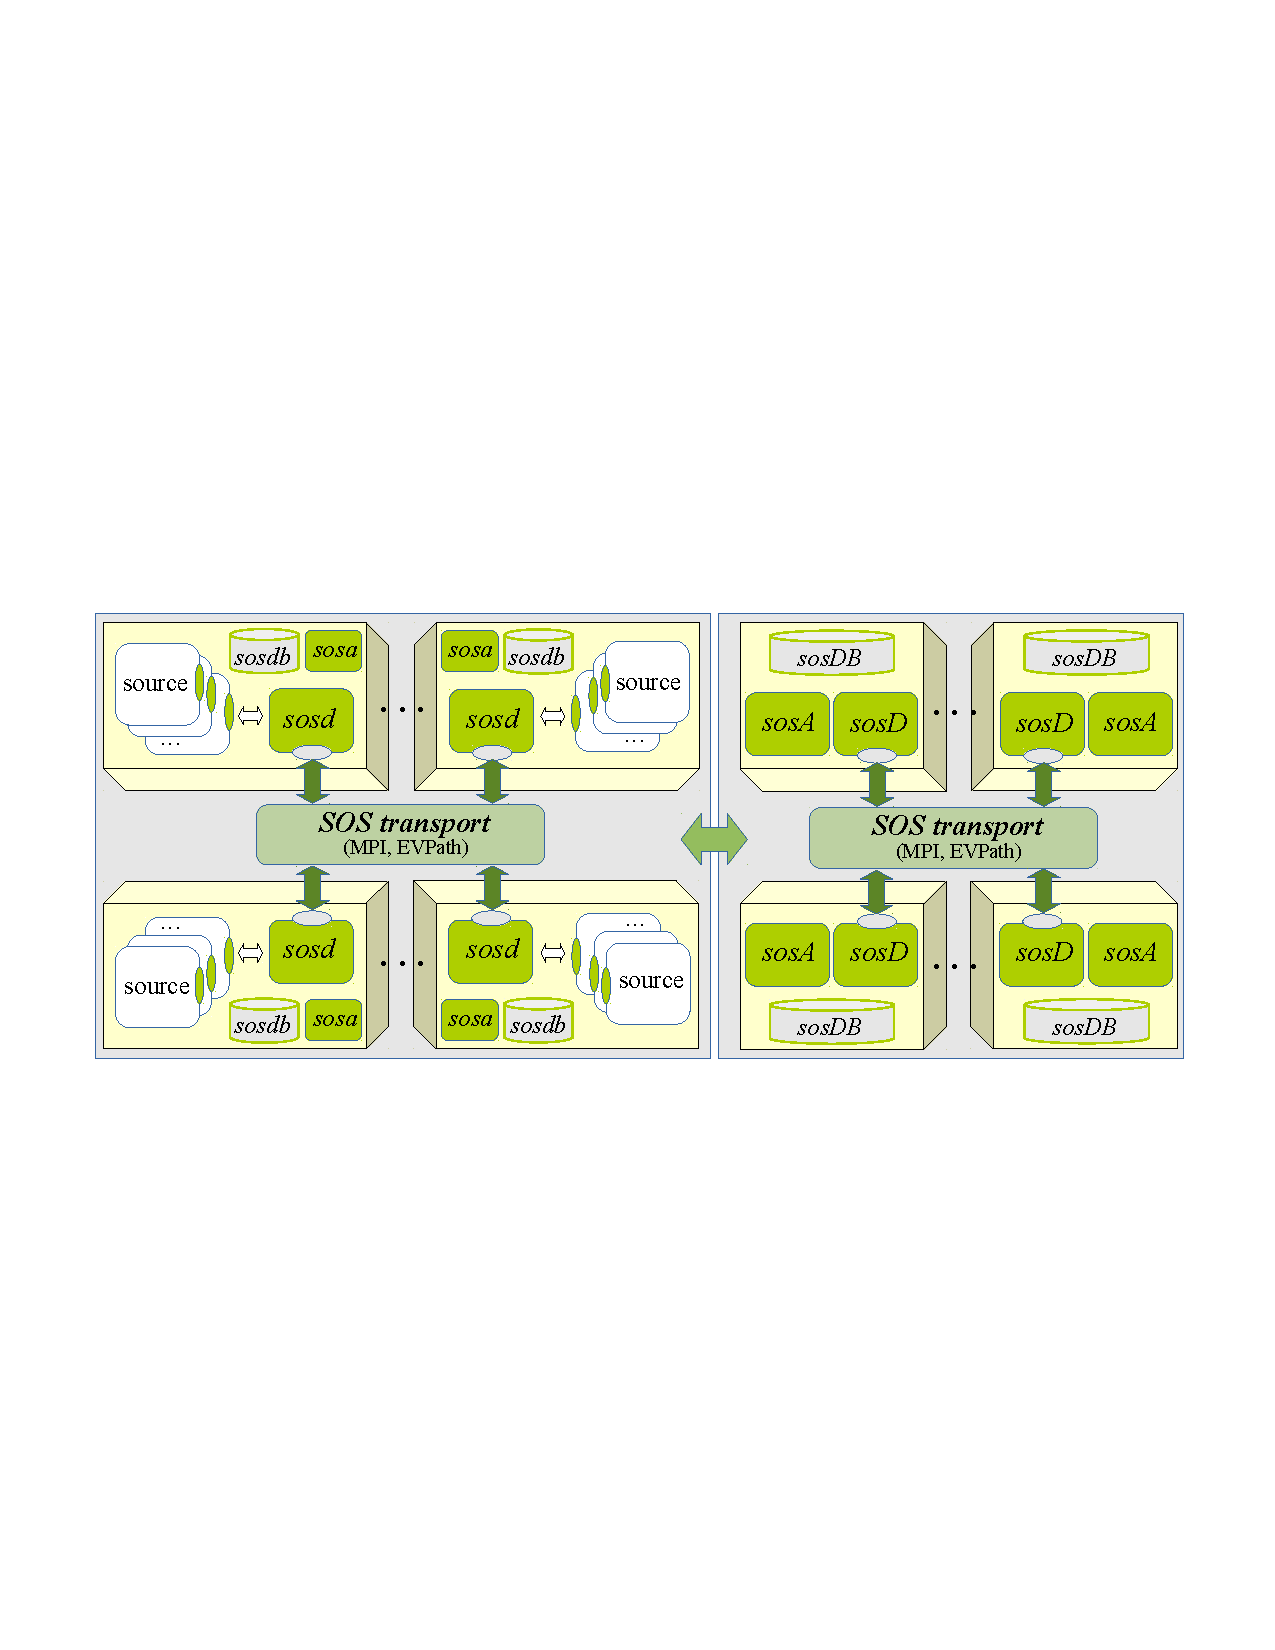
\includegraphics[width=5in]{images/sos.pdf}
  \caption{SOSflow Internal Topology}
  \label{fig_sim}
\end{figure*}
%%%%%



%%%%%%%%%%%%%%%%%%%%%%%%%%%%%%%%%%%%%%%%%%%%%%%%%%%%%%%%%%%%%%%%%%%%%%%%%%%%%%
%%%%%%%%%%%%%%%%%%%%%%%%%%%%%%%%%%%%%%%%%%%%%%%%%%%%%%%%%%%%%%%%%%%%%%%%%%%%%%
%%%%%%%%%%%%%%%%%%%%%%%%%%%%%%%%%%%%%%%%%%%%%%%%%%%%%%%%%%%%%%%%%%%%%%%%%%%%%%

\section{Semantic Performance Model}

%%%%%
Traditionally, HPC research into enhancing performance has been
focused on low-level efficiency of an application or library on some
particular mechine, with tools like TAU bringing HPC developers ever
closer to optimal runs on specific machines.
%
Higher-level systems like TACC Stats \cite{evans2014comprehensive}
allow the tracking and exploration of execution wall-time for
applications compiled using various library versions.
%
The popular Lightweight Distributed Metric System (LDMS)
\cite{agelastos2014lightweight} provides basic integration of multiple
modalities of data in real-time, triggering program invocation or
shaping work allocation across a cluster as informed by network
congestion statistics, and other hybridized or meta-execution data
points.
%%%%%

%%%%%
These tools (and many others) are fast, well-researched, funded, and
they are out there running and very popular already.
%
Unfortunately, \textit{they're solving yesterday's problem tomorrow},
and are firmly grounded in the classic HPC ways of modeling
performance.
%
High-level modeling, in the current jargon, is far too hands-off and
impersonal to be of much general use.
%
Users of such codes have to hard-wire every bit of actual
functionality as a special case, and only by doing so for every
possible use case, for every possible application, for each possible
allocation configuration, can they learn something that is in the end
of no use to anyone but them, right at that time and at no other
time.
%
Worse, as earlier sections outlined, those high-level codes are
actually low-level: They have loosely-coupled components that are
voluntarily participated with, but \textit{everything that those
  components gather and operate over is an empty low-level matter of
  fact} such as latency or binary signature.
%%%%%

%%%%%
Low-level metrics are naturally suited for off-line episodic
performance analysis of individual workflow components.
%
Such deep instrumentation is necessarily invasive and can dictate
rather than capture the observed performance of the instrumented
application when it is run at scale or required to engage in
significant amounts of interactivity.
%
Doing principle components analysis on unconditioned data is also
computationally expensive.
%
Though few values in SOSflow are required to be marked up with
specific metadata, every specifier that can be assigned to a value
will flow with it through the entire runtime and will be made
available to any of the analytics modules.
%%%%%

%%%%%
It is increasingly challenging for static analysis of low-level
features and decontextualized raw codes to produce insight into the
run-time performance of some arbitrary complex workflow.
%
A higher-level approach is required to characterize and reason about
the emergent properties of a large scientific code.
%
Industrial-grade parallel software simulations are interacting
asynchronously across a distributed HPC cluster that is typically
shared with many other users.
%
New ways of describing and comparing scientific workflows are clearly
needed, especially when considering the extreme scales of parallelism
to which scientific workflows are being driven.
%%%%%


%-----------------------------------------------------------------------------

\subsection{The Invariant Meaning of Codes}

%%%%%
Visually, figures are revealed by their background: they break up the
continuity of the background and stand-out in the world.
%
By defining an invariant background for performance observations to be
set off against, the meaning in the codes, the partially summed yet
variously disanalogous sets of observed metrics from a system as a
whole, can be mapped over each other according to a set of organizing
principles that both are individually, and become corporately, an
invariant for that particular complex computation.
%
It doesn't only matter that something is a double precision floating
point, it matters that it holds a measure of time, and it matters that
it's the time something stopped, rather than a simple sample.
%
It doesn't only matter that a process uses a lot of threads, it
matters that it is running well on a machine with a lot of thread
processing cores.
%
It isn't obviously significant for a task to be parameterized by an
auto-tuning algorithm to increased the rate of one of its outputs
rather than other targets, like reducing node memory use, or
increasing the degree of paralellism, unless it is clear that
\textit{something in its output} is being consumed at a great rate
through unsaturated network connections.
%
\textbf{It is only by observing all of these meaningful
  \textit{natures}, \textit{purposes}, and \textit{activities}, that
  the complexity can be properly reasoned about, that the \textit{true
    figure of performance} can be revealed.}
%
It is only with a proper run-time and annotation framework that this
reasoning can take place in a computationally feasible way.
%%%%%

%%%%%
In a very basic sense, so long as it holds that with a certain input a
particular result will be output the same, there is something else
unchanging about a simulation, nomatter how it is tuned or allocated
or configured for a run: the meaning of what happened.
%
Whether a simulation is executing as a single process on a single
node, or billions of independent tasks in a cloud computing
environment, the meaning of what is being computed holds the
same.
%
Though this point may seem fine if not obtuse in this context, the
concept of \textit{invariant meaning} is central to a properly useful
Workflow Performance Model: It must be a Semantic Performance Model.
%%%%%

%%%%%
At extreme scales, on line detection and attribution of meaningful
variability in the performance of a scientific workflow will simply
\textit{require} well-annotated metadata to facilitate "apples to
apples" comparisons driven by unsupervised machine learning rather
than a priori developer knowledge or slow offline centralized
analysis.
%
In the face of wild performance variance across byzantine parameter
spaces, hardware allocations, software libraries, and dynamic
interactions, this kind of meaning invariance is the only ground
truth, the only practical measure of what has been observed.
%
With meaning invariance properly worked into the observation and
analytics structure, real-time systems will be able to efficiently
discover, annotate, share, and potentially even optimize a code's
sensitivity to a particular cluster or allocation, its propensity for
creating and propagating performance variability into other unrelated
parts of the system, and then finally pinpoint the lower-level
software mechanics giving rise to the higher level phenomenon.
%%%%%

%-----------------------------------------------------------------------------

\subsection{Levels of Description and "The View from Anywhere"}
%%%%%
Not wanting to limit \textit{a priori} what component or layer of the
workflow \textit{is allowed to be interesting} during the analysis of
performance, the SOS workflow performance model flourishes when
populated by a diversity of information sources, each providing
metrics with tailored metadata, logical events like notes about things
happening inside the simulation they are running, and concrete events
-- all arriving in real-time from many different layers of activity in
a workflow:
%
\begin{itemize}
      %
    \item Workflow
      %
    \item Simulation
      %
    \item Application
      %
    \item Algorithm
      %
    \item Libraries
      %
    \item Environment
      %
    \item Developer Tools
      %
    \item Operating System
      %
    \item Node Hardware
      %
    \item Network
      %
    \item Enclave
      %
    \item Cluster
      %
    \item Epoch
      %
\end{itemize}
%%%%%

%%%%%
Each of these layers constitutes a level of description for the
overall system performance, and the performance of any component is a
composite of slices through any layers that component is participating
in or contingent on.
%
It becomes a tantalizing possibility that events and metrics stored in
SOS for a very narrow end-user purpose wind up supporting critical
inferences used to discover patterns and features of system-wide
utility.
%
If a developer finds she can get some benefit by using the SOSflow
toolkit for a once-off research project, the metrics that are then
even \textit{accidentally} contributed might turn out to have been
unpolished research gems hiding in tomorrow's data stores.
%%%%%

%%%%%
Metrics from multiple layers can be correlating to yield interesting
perspectives on the observed performance of specific software
components.
%
As a trivial example, something at the Simulation layer produces data
representing the evolution of a data set over N seconds of simulated
time, and the Application layer requires M seconds of real-world
computation to yield that data, the relationship between N and M could
be a valid performance metric to report, compare across runs,
calculate real-dollar-cost to compute, or attempt to generally
optimize through parameter convergence.
%
A key takeaway here is: \textit{The particular purpose for gathering
  that data does NOT need to be known in advance}, sampling would not
need to be programmed into the application by hand every time a
researcher or performance tuning engine asked a question, rather,
on-demand queries could be run to discover such correlations and
features of performance at any time, or \textit{even in real-time} as
fresh data is flowing in.
%
It is also importantly to note that components of a layer not only can
contribute metrics, they (and other components at that layer) are
targets for feedback and control.
%%%%%

%-----------------------------------------------------------------------------

\subsection{Semantics}

All information that is gathered by the monitoring system should be
annotated as richly as possible to maximize its usefulness when
performing analytics.
%
Hand-annotated codes will have the most to offer an analytics engine,
values that are tracked will be able to carry a full spectrum of
high-level tags that express what that data means and what could be
expected of it, in structures preserving some human programmer or
user's understanding.
%
Capturing this metadata using semantic markups with action-grounded
significance has the benefit of their being compatible with
unsupervised machine-learning tests for significance and other
advanced analysis techniques that will ultimately be able to converge
on outcomes desirable to the human developers and users of the system.
%%%%%

%%%%%
Not everything has to be surgically annotated for it to be of benefit.
%
Any episodic performance measurement, such as run-time TAU
instrumentation and results, can also be injected into the SOSflow engine, and the
SOSflow runtime is able to differentiate from information pushed
directly by a layer, and information that is being captured by finer-grained
middleware tools that are only equipped to signify generic facts of matter.
%%%%%

%%%%%
Semantic information is local to the pub handle created by a source
that is contributing to SOSflow.
%
Sources can create multiple pubs to distinctly represent potential
compound or complex roles.
%
Pubs carry their own pub-wide semantic markups, including the origin
layer, a role within that layer, and information about the node that
the source process is running on.
%
Semantic markups are then nested inside of the pub handle, as each
value that is pushed into the SOSflow system through a pub handle also
comes with a rich set of high-level semantic tags that stay affiliated
with it over time, and various ephemeral notions to color the rigid
meaning invariance with motivating indicators of changes in state,
such as the \textit{mood} of a value, which can be: DEFAULT, GOOD,
BAD, UGLY.
%
The ephemeral indicators are mere hints, motivators, not themselves
signifiers of meaning but more the glue between meanings revealed by
the coocurrence of change.
%
Sometimes it matters less what changed into what, than that something
changed at all.
%%%%%

While deep off-line data analytics can reveal \textit{unforseen correlations}
between various aspects of the workflow or the data set it is
operating over, the interest in real-time analytics and performance
tuning gives value to expressing "relationship hints" between values
tracked by the system.
%
These hints can be used to direct in situ analytics efficiently, to
narrow the parameter space into something tractable without
interfereing with the principle computational load of a given
node.
%
Expressed relationship hints are a double-edged sword, as one of the
draws of the performance model is that nobody has to know the big
picture in order to get some value out of it.
%
Rather than call them relationship \textit{rules} we say
\textit{hints} and suggest that unless someone really knows what
they're looking for, such as when they write an online analytics
module for their own code, the hints functionality can be safely
ignored.
%
When one's analytics are looking to identify specific deviations from
predictable expectations; anything that can be overtly identified as
an expectation for a value can be used to narrow the search space when
doing unsupervised machine learning over gathered workflow performance
data.
%
Such accessory features are supported but not required, or even truly
emphasized.
%%%%%

%-----------------------------------------------------------------------------

\subsection{The Utility a Comprehensive Semantic Performance Model}

%%%%%
At this point it is safe to leave it to the reader's imagination to
ponder the possible utility of a mature Semantic Performanice Model /
Workflow Performance Model.
%
Especially given that there is an extant implementation of it that
functions with relative efficiency and is capable of operating online
and in user space on today's commodity HPC hardware.
%
The exascale architectures will likely prove even more effective
hosts: Their incredible computational density and scale has proven
difficult to completely saturate with work that is purely organic to
any given problem at hand, so there will likely be plenty of available
computational resources to direct towards these higher-level systems.
%%%%%

%%%%%
Some specific immediate perks would be enhancements to:
%
\begin{itemize}
      %
    \item \textbf{Attribution}: Point the blame at the offending job
      or shared resource.
      % 
      Developers don't always know their own code so well, or how it
      will interact with a total system, so capturing from a wide
      array of sources will help eliminate the guessing game when it
      comes time to grab the pitchforks.
      %
    \item \textbf{Accuracy}: If you've got data showing consistent behavior on
      certain allocations, and bad behavior when certain hardware resources
      get involved, you've got a better sense about what part of your
      fate you can control, about what variation is yours, and what comes
      from the Lord.
      %
    \item \textbf{Resource Requirement Prediction}: 2 + 2 isn't always
      4 when it comes to guessing about the perturbation of processes
      interacting in dynamical systems.
      %
      Being aware of each others presence through shared real-time
      self-reporting will allow applications to adapt themselves and
      administrators to preemptively allocate to promote positive
      disruption of learned negative performance patterns.
      %
    \item \textbf{Automated Component Performance Tuning}: Nobody
      wants conflicting optimizer purposes, and having them working
      from a global perspective will need to show where the true
      systemic hotspots really are, and not depend on an individual
      developers being a total system expert or a selfless
      non-optimizer.
      %
\item \textbf{Intelligent Compiler Hints}: Anything that is learned from all
      this richly annotated performance data can ultimately be tied back
      into intelligent compilers and IDE's.
      %
      That way a new hire doesn't have to burn 1,000,000 hours of
      allocation to learn that they've just re-created the exact code
      pattern or data structure that led to last year's round of
      layoffs and funding cuts.
      %
    \item \textbf{Intelligent Job Scheduling}: Because ``optimum job
      scheduling'' is not a univocal term.
      %
\end{itemize}
%%%%%

%%%%%
The SOS workflow performance model is still being refined, and more
serious demonstrations are needed in order to convince people that
their cluster should have an always-on observation and analysis
platform.
%
Perhaps all an admin wants to do is run 25-year old Fortran codes as
inefficiently and as often as possible, so long as the support phone
never rings.
%
We suspect that given the peculiar nature of distributed mobile
computing paired with the looming tectonic shift to exascale compute
platforms, SOS's model will prove timely and deeply beneficial to a
variety of interests.
%%%%%

%\todofileend{030\_sos\_model.tex}
